\subsection{\RU{Чтение за пределами массива}\EN{Reading behind array bounds}}

\RU{Итак, индексация массива ~--- это просто \IT{массив\lbrack{}индекс\rbrack}.  % TODO как-то плохо отображаются []
Если вы присмотритесь к коду, в цикле печати значений массива через \printf вы 
не увидите проверок индекса, \IT{меньше ли он двадцати?} 
А что будет если он будет 20 или больше? 
Эта одна из особенностей \CCpp, за которую их, собственно, и ругают.}
\EN{So, array indexing is just \IT{array\lbrack{}index\rbrack}.
If you study generated code closely, you'll probably note missing index bounds checking,
which could check index, \IT{if it is less than 20}.
What if index will be 20 or greater?
That's the one \CCpp feature it is often blamed for.}

\RU{Вот код который и компилируется и работает:}
\EN{Here is a code successfully compiling and working:}

\lstinputlisting{patterns/13_arrays/2_BO/r.c}

\RU{Вот в это}\EN{Compilation results} (MSVC 2008):

\lstinputlisting{patterns/13_arrays/2_BO/r_msvc.asm}

\RU{У меня оно при запуске выдало вот это:}\EN{I'm running it, and I got:}

\begin{figure}[h]
\centering
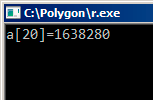
\includegraphics[scale=0.66]{patterns/13_arrays/2_BO/olly_r3.png}
\caption{\olly: \RU{вывод в консоль}\EN{console output}}
\label{fig:array_BO_olly_r3}
\end{figure}

\RU{Это просто \IT{что-то}, что волею случая лежало в стеке рядом с массивом, 
через 80 байт от его первого элемента.}
\EN{It is just \IT{something}, occasionally lying in the stack near to array, 80 bytes from its first element.}

\index{\olly}
\RU{Попробуем узнать в \olly, что это за значение}\EN{Let's try to find out using \olly, 
where this value came from}.
\RU{Загружаем и находим это значение, находящееся точно после последнего элемента массива}
\EN{Let's load and find a value located right after the last array element}:
\figref{fig:array_BO_olly_r1}.
\RU{Что это за значение}\EN{What is this}? 
\RU{Судя по разметке стека, это сохраненное значение регистра EBP}\EN{Judging by stack layout,
this is saved EBP register value}.
\RU{Трассируем далее, и видим как оно восстанавливается}\EN{Let's trace further and see, how
it will be restored}:
\figref{fig:array_BO_olly_r2}.

\RU{Действительно, а как могло бы быть иначе? Компилятор мог бы встроить какой-то код, 
каждый раз проверяющий индекс на соответствие пределам массива, как в языках программирования 
более высокого уровня\footnote{Java, Python, и т.д.}, что делало бы запускаемый код медленнее.}
\EN{Indeed, how it could be done differently?
Compiler may generate some additional code for checking index value to be always
in array's bound (like in higher-level programming languages\footnote{Java, Python, etc})
but this makes running code slower.}

\begin{figure}[H]
\centering
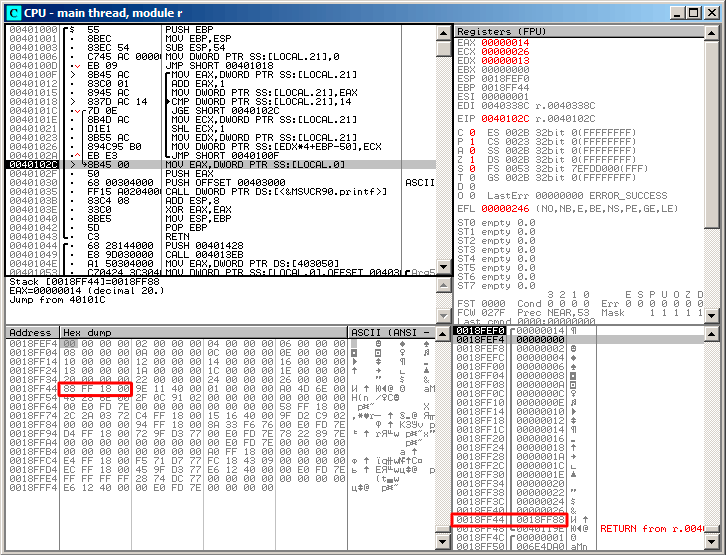
\includegraphics[scale=\FigScale]{patterns/13_arrays/2_BO/olly_r1.png}
\caption{\olly: \RU{чтение 20-го элемента и вызов \printf}\EN{reading of 20th element and execution of \printf}}
\label{fig:array_BO_olly_r1}
\end{figure}

\begin{figure}[H]
\centering
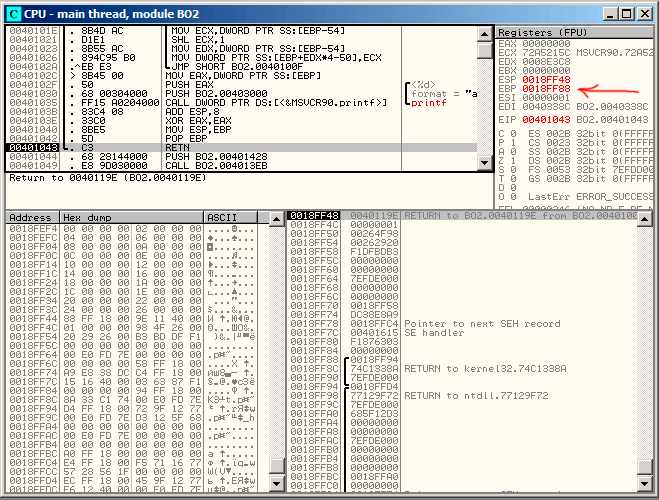
\includegraphics[scale=\FigScale]{patterns/13_arrays/2_BO/olly_r2.png}
\caption{\olly: \RU{восстановление EBP}\EN{restoring value of EBP register}}
\label{fig:array_BO_olly_r2}
\end{figure}
